%
%   Chapter Experiments
%
%   Yong-Siang Shih
%   R.O.C.104.07
%
\chapter{Experiments}
\label{c:exp}

\section{Discourse Usage Disambiguation}
\label{c:discourse-usage-exp}

In this section, we describe our investigation
on discourse usage disambiguation. We evaluate our models using
10-fold cross-validation. The 2,342 paragraphs are divided  into 10 folds
while keeping the distribution of the number of explicit relations
in each paragraph roughly equal. Most of the related works only
deal with connective components, so we will also use the 2,131 annotated
components to evaluate our models.
The precision, recall, and F1 score for the positive instances are computed
for each fold, and the average is reported.


We firstly experiment with different types of word embeddings for
the VECTOR features. We use Logistic Regression as our classifier
and use VECTOR as the only features. The results are
shown in Table~\ref{t:recognition-vectors} below. 

\begin{table}[ht]
\centering
\begin{tabular}{|l|c|c|c|}
\hline

\bf Features        & \bf Precision & \bf Recall & \bf F1-Score \\ \hline
    GLOVE           &     77.95     &     75.77  &     76.79    \\ \hline
    SKIPGRAM        & \bf 78.33     &     76.28  & \bf 77.25    \\ \hline
    CBOW            &     75.08     &     73.97  &     74.48    \\ \hline
    GLOVE+SKIPGRAM  &     77.82     & \bf 76.57  &     77.15    \\ \hline
    GLOVE+CBOW      &     74.63     &     73.79  &     74.14    \\ \hline
    SKIPGRAM+CBOW   &     74.56     &     73.55  &     74.01    \\ \hline
    All             &     74.91     &     73.46  &     74.12    \\ \hline

\end{tabular}
\caption{\label{t:recognition-vectors} Performance of discourse usage
disambiguation on component level using different word embeddings for
the VECTOR features. }
\end{table}


In particular, GLOVE is a 400-dimensional vector trained using the
toolkit provided by \cite{pennington2014glove} while SKIPGRAM and
CBOW are trained using word2vec~\citep{mikolov2013efficient} with
continuous skip-gram model and continuous bag-of-words model,
respectively, as discussed in Chapter~\ref{c:datasets}. SKIPGRAM
yields the best results on both precision and F1-score. We have
tried concatenating different embeddings but the performance does not
improve. Therefore, we will only use SKIPGRAM for the remaining experiments.

We also use the same 10-fold to evaluate different features we proposed.
The results are shown in Table~\ref{t:recognition-features}. SIKIPGRAM
is the most powerful feature. Combining all features gives the best
results.

\begin{table}[h]
\centering
\begin{tabular}{|c|c|c|c|}
\hline

\bf Features        & \bf Precision & \bf Recall & \bf F1-Score \\ \hline
    P \& N          &     74.52     &     45.02  &     55.96    \\ \hline
    POS             &     75.47     &     65.76  &     70.24    \\ \hline
    NUM             &     68.39     &     22.20  &     33.30    \\ \hline
    SKIPGRAM        &     78.33     &     76.28  &     77.25    \\ \hline
    All-P\& N       &     79.09     &     76.97  &     77.99    \\ \hline
    All-POS         &     78.90     &     76.64  &     77.73    \\ \hline
    All-NUM         &     79.42     & \bf 77.44  &     78.40    \\ \hline
    All-SKIPGRAM    &     77.89     &     68.70  &     72.96    \\ \hline
    All             & \bf 79.92     & \bf 77.44  & \bf 78.64    \\ \hline

\end{tabular}
\caption{\label{t:recognition-features} Performance of discourse usage
disambiguation for connective components by different features. }
\end{table}


We use Scikit-Learn library~\citep{scikit-learn} to experiment with
several different learning models with default parameters using all the features.
Table~\ref{t:recognition-models} shows the results. The F1 score for Logistic
Regression is the highest.


\begin{table}[ht]
\centering
\begin{tabular}{|l|c|c|c|}
\hline

Model                  &     Precision &     Recall &     F1-Score                 \\ \hline
Gaussian Naive Bayes   &     42.35     & \bf 92.17  &     58.02\textsuperscript{*} \\ \hline
SVM with RBF kernel    &     80.00     &     69.84  &     74.55\textsuperscript{*} \\ \hline
SVM with linear kernel &     75.75     &     74.71  &     75.20\textsuperscript{*} \\ \hline
Decision Tree          &     74.85     &     73.83  &     74.98\textsuperscript{*} \\ \hline
Random Forest          & \bf 83.25     &     72.09  &     77.20\textsuperscript{*} \\ \hline
Logistic Regression    &     79.92     &     77.44  & \bf 78.64\textsuperscript{!} \\ \hline

\end{tabular}
\caption{\label{t:recognition-models} Performance of discourse usage
disambiguation on component level using different learning models. }
\end{table}


We summarize our results in Table~\ref{t:recognition-methods} and
compare with various related work. The first model is the method we described above
using all features with Logistic Regression. For pipeline-by-component,
we take the connective components extracted from the previous model, and try to
identify the correct linkings between the components as described in Section~\ref{c:pipeline1}.
The component candidates that fail to form a connective are eliminated.
Some spurious candidates are removed in this process. However, it also removes some
correct components, so the resulting F1 score does not improve. Comparatively,
pipeline-by-connective yields a slightly better result. As described in
Section~\ref{c:pipeline2}, we use each connective candidate as an instance and
disambiguate discourse and non-discourse usages on the connective level.
The improvement suggest that linking information may help discourse usage disambiguation.
Though further investigation is needed to confirm the idea.

We also compare our results with the models from \cite{li2015automatic} as they use the
same dataset as us. The best results for Maximum Entropy and Decision Tree classifiers with
automatic parsing tree features are selected. We use the 12,526 connective components candidates
extracted by string matching with connective lexicon as our basis to compute the accuracy in order
to compare with their work. Our models perform significantly better by a large margin.

We also list the results from \cite{zhou2012cross} and \cite{li2014cross} on different
datasets. Though it's not directly comparable with our work, the performance is similar.

\begin{table}[ht]
\centering
\begin{tabular}{|c|c|c|c|c|}
\hline

\bf Features                  & \bf Precision & \bf Recall & \bf F1-Score & \bf Accuracy \\ \hline
    logistic regression       &     79.92     &     77.44  &     78.64    &     92.84    \\ \hline
    pipeline-by-component     & \bf 81.84     &     75.66  &     78.60    & \bf 92.96    \\ \hline % length+logistic
    pipeline-by-connective    &     77.27     & \bf 80.45  & \bf 78.81    &     92.61    \\

\hhline{|=|=|=|=|=|}

    Li et al. maximum entropy &     78.80     &     61.80  &     69.20    &     87.20    \\ \hline
    Li et al. decision tree   &     56.80     &     49.60  &     52.30    &     88.40    \\

\hhline{|=|=|=|=|=|}

    Zhou et al.               &               &            &     79.33    &     70.43    \\ \hline
    Li, M \& N                &     78.57     &     81.48  &     80.00    &     82.04    \\ \hline

\end{tabular}
\caption{\label{t:recognition-methods} Performance of discourse usage
disambiguation for connective components by methods. }
\end{table}


\section{Discourse Linking Disambiguation}
\label{c:linking-exp}

In this section, we discuss our investigation on linking ambiguities between connective components. Evaluation is done with the 1,813 connective instances. The same 10-fold
for paragraphs is used for the experiments.

We first examine the pipeline-by-component approach and assume all connective
components are correctly identified so we can evaluate linking disambiguation
independently. We use logistic regression
to get the probability for each connective candidate to be correct and greedily
accept non-overlapping candidates. We break ties by the positions of their components.
Left-most candidates are accepted first. Experiments are done to investigate whether
similar features are also useful for linking disambiguation and 
Table~\ref{t:perfect-features} shows the results. We found that
the only features that perform well are the NUM features. Further investigation
reveals that using the length as the only feature actually performs better.
In fact, if we simply order each candidate by their lengths and the positions,
accepting candidates that have most components and left-most positions, we could
reach the best results.


\begin{table}[h]
\centering
\begin{tabular}{|c|c|c|c|}
\hline

\bf Features            & \bf Precision & \bf Recall & \bf F1-Score \\ \hline
    P \& N              &     92.11     &     92.76  &     92.43    \\ \hline
    POS                 &     88.36     &     91.55  &     89.93    \\ \hline
    NUM                 & \bf 95.59     & \bf 96.58  & \bf 96.08    \\ \hline
    SKIPGRAM            &     88.30     &     91.94  &     90.08    \\ \hline
    All-P \& N          &     94.57     &     96.13  &     95.35    \\ \hline
    All-POS             &     93.88     &     95.53  &     94.70    \\ \hline
    All-NUM             &     90.82     &     93.37  &     92.08    \\ \hline
    All-SKIPGRAM        &     94.86     &     96.19  &     95.52    \\ \hline
    All                 &     94.47     &     96.13  &     95.29    \\

\hhline{|=|=|=|=|}

    Left-first          &     85.89     &     91.01  &     88.37    \\ \hline
    Length              &     97.59     &     96.04  &     96.81    \\ \hline
    Order by length     & \bf 97.71     & \bf 96.15  & \bf 96.92    \\

\hhline{|=|=|=|=|}
% length then this

    P \& N              &     97.26     &     95.60  &     96.42    \\ \hline
    POS                 &     97.48     &     95.82  &     96.64    \\ \hline
    NUM                 & \bf 98.48     & \bf 96.92  & \bf 97.69    \\ \hline
    SKIPGRAM            &     97.87     &     96.37  &     97.10    \\ \hline
    All-P \& N          &     97.81     &     96.25  &     97.02    \\ \hline
    All-POS             &     97.81     &     96.25  &     97.02    \\ \hline
    All-NUM             &     97.54     &     96.03  &     96.78    \\ \hline
    All-SKIPGRAM        &     97.92     &     96.36  &     97.13    \\ \hline
    All                 &     97.81     &     96.25  &     97.02    \\


\end{tabular}
\caption{\label{t:perfect-features} Performance of discourse usage
disambiguation for connective by different features. }
\end{table}


Therefore, we incorporate these methods and rank each candidate using the following
criteria respectively:

\begin{enumerate}
    \item the length, the more components the higher the score
    \item the score obtained by logistic regression
    \item the positions of components, left is better
\end{enumerate}

Table~\ref{t:perfect-length} shows the results. We compare different features
with a baseline that only use positions for ranking (Left-first) and another
baseline using both lengths and positions (Order by length). NUM features gives
a slightly better result.

\begin{table}[ht]
\centering
\begin{tabular}{|c|c|c|c|}
\hline

\bf Methods             & \bf Precision & \bf Recall & \bf F1-Score \\ \hline
    Left-first          &     85.89     &     91.01  &     88.37    \\ \hline
    Order by length     & \bf 97.71     & \bf 96.15  & \bf 96.92    \\

\hhline{|=|=|=|=|}
% length then this
    P \& N              &     97.26     &     95.60  &     96.42    \\ \hline
    POS                 &     97.48     &     95.82  &     96.64    \\ \hline
    NUM                 & \bf 98.48     & \bf 96.92  & \bf 97.69    \\ \hline
    SKIPGRAM            &     97.87     &     96.37  &     97.10    \\ \hline
    All-P \& N          &     97.81     &     96.25  &     97.02    \\ \hline
    All-POS             &     97.81     &     96.25  &     97.02    \\ \hline
    All-NUM             &     97.54     &     96.03  &     96.78    \\ \hline
    All-SKIPGRAM        &     97.92     &     96.36  &     97.13    \\ \hline
    All                 &     97.81     &     96.25  &     97.02    \\ \hline


\end{tabular}
\caption{\label{t:perfect-length} Performance of discourse usage
disambiguation for connective by different features. }
\end{table}


We also carry out the same experiments when the component candidates are automatically
extracted as discussed in Section~\ref{c:discourse-usage-exp}. However, the results
are different. As shown in Table~\ref{t:pipeline-features}, when using scores
predicted by logistic regression, All-SKIPGRAME gives the best results. Also,
the its performance is better than the Order by length baseline.

\begin{table}[h]
\centering
\begin{tabular}{|c|c|c|c|}
\hline

\bf Features            & \bf Precision & \bf Recall & \bf F1-Score \\ \hline
    P \& N              &     72.42     &     70.52  &     71.45    \\ \hline
    POS                 &     70.47     &     70.47  &     70.46    \\ \hline
    NUM                 &     73.08     &     71.80  &     72.41    \\ \hline
    SKIPGRAM            &     69.35     &     69.58  &     69.46    \\ \hline
    All-P \& N          &     73.55     &     72.45  &     72.99    \\ \hline
    All-POS             &     73.33     &     72.24  &     72.77    \\ \hline
    All-NUM             &     72.04     &     71.13  &     71.56    \\ \hline
    All-SKIPGRAM        & \bf 74.00     & \bf 72.67  & \bf 73.31    \\ \hline
    All                 &     73.79     &     72.40  &     73.07    \\

\hhline{|=|=|=|=|}

    Left-first          &     68.25     &     69.70  &     68.96    \\ \hline
    Length              &     74.47     &     71.03  &     72.70    \\ \hline
    Order by length     & \bf 74.53     & \bf 71.09  & \bf 72.75    \\

\hhline{|=|=|=|=|}


    P \& N              &     74.38     &     70.86  &     72.57    \\ \hline
    POS                 &     74.45     &     70.98  &     72.66    \\ \hline
    NUM                 &     74.93     &     71.52  &     73.18    \\ \hline
    SKIPGRAM            &     75.17     &     71.69  &     73.38    \\ \hline
    All-P \& N          &     75.37     &     71.85  &     73.56    \\ \hline
    All-POS             &     75.60     &     72.02  &     73.76    \\ \hline
    All-NUM             &     74.92     &     71.41  &     73.11    \\ \hline
    All-SKIPGRAM        &     75.53     &     71.91  &     73.66    \\ \hline
    All                 & \bf 75.66     & \bf 72.08  & \bf 73.81    \\

\end{tabular}
\caption{\label{t:recognition-features} Performance of discourse usage
disambiguation for connective components by different features. }
\end{table}


Comparatively, when we use length and scores together, using all features gives
best results as shown in Table~\ref{t:pipeline-length}.

\begin{table}[ht]
\centering
\begin{tabular}{|c|c|c|c|}
\hline

\bf Features            & \bf Precision & \bf Recall & \bf F1-Score \\ \hline
    Left-first          &     68.25     &     69.70  &     68.96    \\ \hline
    Length              &     74.47     &     71.03  &     72.70    \\ \hline
    Order by length     & \bf 74.53     & \bf 71.09  & \bf 72.75    \\

\hhline{|=|=|=|=|}


    P \& N              &     74.38     &     70.86  &     72.57    \\ \hline
    POS                 &     74.45     &     70.98  &     72.66    \\ \hline
    NUM                 &     74.93     &     71.52  &     73.18    \\ \hline
    SKIPGRAM            &     75.17     &     71.69  &     73.38    \\ \hline
    All-P \& N          &     75.37     &     71.85  &     73.56    \\ \hline
    All-POS             &     75.60     &     72.02  &     73.76    \\ \hline
    All-NUM             &     74.92     &     71.41  &     73.11    \\ \hline
    All-SKIPGRAM        &     75.53     &     71.91  &     73.66    \\ \hline
    All                 & \bf 75.66     & \bf 72.08  & \bf 73.81    \\ \hline

\end{tabular}
\caption{\label{t:pipeline-length} Performance of discourse usage
disambiguation for connective components by different features. }
\end{table}


This seems to suggest that these features may perform better when there are
spurious component candidates because they can be used to eliminate some of
these candidates.  Thus, we try a different model as shown in
Table~\ref{t:classify-features} and obtain better results.

\begin{table}[ht]
\centering
\begin{tabular}{|c|c|c|c|}
\hline

\bf Features            & \bf Precision & \bf Recall & \bf F1-Score \\ \hline
    P \& N              &     48.73     &     75.73  &     59.26    \\ \hline
    POS                 &     62.64     &     70.98  &     66.52    \\ \hline
    NUM                 &     46.80     & \bf 78.87  &     58.71    \\ \hline
    SKIPGRAM            &     69.20     &     72.79  &     70.93    \\ \hline
    All-P \& N          &     72.24     &     76.48  &     74.27    \\ \hline
    All-POS             &     72.43     &     76.59  &     74.43    \\ \hline
    All-NUM             &     71.86     &     73.85  &     72.83    \\ \hline
    All-SKIPGRAM        &     64.09     &     76.37  &     69.65    \\ \hline
    All                 & \bf 73.30     &     76.75  & \bf 74.97    \\ \hline


\end{tabular}
\caption{\label{t:classify-features} Performance of discourse linking
disambiguation for connectives by different features.} This is done by
treating each connective as an instance then classify their discourse usage
by logistic regression. Aftwards, we rank each candidate by length and their
logistic probability and reject overlappped ones.
\end{table}



We also try to adjust the threshold to eliminate the candidates and found
that our model obtain similar F1 scores across different thresholds as
shown in Figure~\ref{i:classify-threshold}.

\begin{figure}[ht]
\centering
    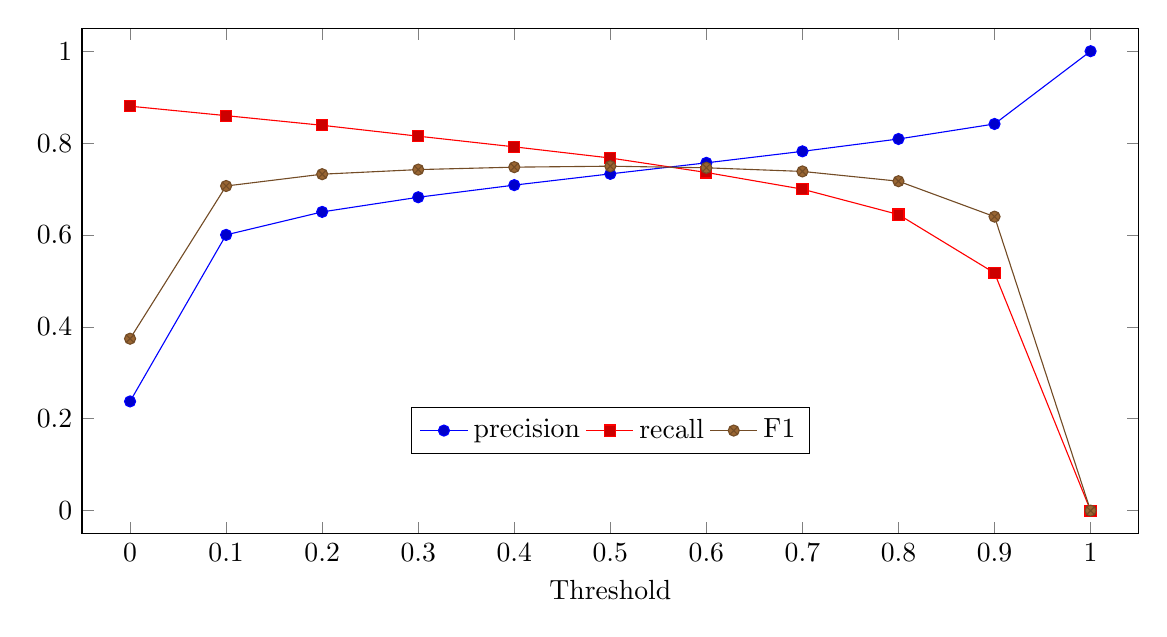
\begin{tikzpicture}
        \begin{axis}[
                height=8cm,
                width=15cm,
                xlabel=Threshold,
                legend style={at={(0.5,0.25)},
                anchor=north,legend columns=-1},
                enlarge x limits=0.05,
                enlarge y limits=0.05,
                xticklabel style={/pgf/number format/assume math mode},
                yticklabel style={/pgf/number format/assume math mode},
            ]
            \addplot+[sharp plot] coordinates
            {
                (0.0,0.2377)
                (0.1,0.6002)
                (0.2,0.6502) 
                (0.3,0.6821) 
                (0.4,0.7085) 
                (0.5,0.7330)
                (0.6,0.7570) 
                (0.7,0.7820) 
                (0.8,0.8089) 
                (0.9,0.8416) 
                (1.0,1.0000)};

            \addplot+[sharp plot] coordinates
            {
                (0.0,0.8803)
                (0.1,0.8597) 
                (0.2,0.8387) 
                (0.3,0.8150) 
                (0.4,0.7918) 
                (0.5,0.7675)
                (0.6,0.7360) 
                (0.7,0.6997) 
                (0.8,0.6445) 
                (0.9,0.5172) 
                (1.0,0.0000)};

            \addplot+[sharp plot] coordinates
            {
                (0.0,0.3742)
                (0.1,0.7066) 
                (0.2,0.7323) 
                (0.3,0.7423) 
                (0.4,0.7476) 
                (0.5,0.7497)
                (0.6,0.7462) 
                (0.7,0.7383) 
                (0.8,0.7170) 
                (0.9,0.6399) 
                (1.0,0.0000)};

            \legend{precision,recall,F1}
        \end{axis}
    \end{tikzpicture}
\caption{\label{i:classify-threshold} Performance for the pipeline system
with different thresholds. }
\end{figure}


\section{Discourse Relation Disambiguation}

10-fold firstly.

We also investigate end-to-end.


\section{Explicit Discourse Relation Argument Extraction}
